\section{Experiment}

\subsection{Appearance Editing}
% Since our method separates the geometry and the appearance, we can easily achieve appearance editing by just editing the record images. We can use InstructPix2Pix ~\cite{brooks2022instructpix2pix} to edit the images by inputting a text prompt. After the recorded images are changed, all the novel trajectories generated using these edited images will be changed automatically since the pseudo frames of the novel trajectories sample colors from these edited images. Although the instruct-pix2pix can only edit images individually, our model can still generate consistent videos because the underlining geoemtry is not changed and still consistent and our video diffusion model can handle the subtle inconsistency of the psuedo frames. Please check the figure [XXX] to see the result of changing the weather into night and rainy day. And please also watch the video in the supplementary materials to check our results. 

Since our method disentangles geometry from appearance, appearance editing can be performed easily by modifying the recorded images. We can leverage SOTA video editing methods, such as VACE~\cite{vace}, Instruct-V2V~\cite{cheng2023consistent}, or other techniques to edit the appearance of recorded images. 
Once the recorded images are altered, all novel trajectories generated from them automatically reflect these changes, as the pseudo-views sample colors directly from the edited images.
This ensures consistent appearance editing across arbitrary camera trajectories.
For example, we can modify the weather in a scene simply by providing a text prompt using Instruct-V2V. Additionally, the mv2v function in the VACE model allows us to alter the appearance of cars. Thanks to recent advances in powerful video editing methods, our approach can leverage these tools to enable versatile editing of driving scenes.
Please refer to Fig.~\ref{fig:teaser} for qualitative results demonstrating appearance edits. We also encourage you to check the supplementary for additional results.

\begin{figure*}
    \centering

    \includegraphics[width=\linewidth]{images/comparison.pdf}

    \caption{Qualitative comparison of novel trajectories with a 3-meter lane shift. In the comparison, the fourth row is shifted to the right, while the others are shifted to the left.}

    \label{fig:comparison}
\end{figure*}


\subsection{Comparison}
\label{sec:comparison}
% We conduct all the experiments on the same test dataset as ReconDreamer ~\cite{Ni2024ReconDreamerCW}. The test dataset is selected from the Waymo validation dataset. Please check the supplementary materials for specific scene IDs and frame numbers. To demonstrate our model's ability to generate high-fidelity novel trajectories, we quantitatively compare our method with several state-of-the-art methods: PVG~\cite{chen2023periodic}, S3gaussian~\cite{huang2024s3gaussian}, DriveDreamer4D~\cite{zhao2024drive}, ReconDreamer~\cite {Ni2024ReconDreamerCW}, and Deformable-GS~\cite{yang2023deformable3dgs}. DriveDreamer4D and ReconDreamer have 3 different implementations, i.e., DriveDreamer4D with PVG, S3gaussian, and Deformable-GS. and ReconDreamer with PVG, S3gaussian, and Deformable-GS. We compared them separately. Since FreeVS~\cite{wang2024freevs} can only generate half of the novel view, we compare it qualitatively. We adopt the metric Novel Trajectory Agent IoU (NTA-IoU) and Novel Trajectory Lane IoU (NTL-IoU), proposed by DriveDreamer4D. We also calculate the FID to measure the differences in feature distribution between novel trajectory images and original trajectory images. To better simulate the real driving cases, we select the line change, which shifts to the left by 0.1 per frame. Since the test segments have 40 frames, the final shift distance is 4 meters. Our method takes 4 progressive steps to achieve the 4-meter shift, i.e., 1 meter shift for a step. The result is shown in the table [XXX]. Our method achieves the highest score on NTA-IoU and NTL-IoU, which means our method can generate novel trajectories with more recognizable vehicles and lines and these vehicles and lines have more accurate locations. Our model also achieves the lowest FID score, which means our method generated more photorealistic results compared with other methods. 

% Since the DriveDreamer4D and ReconDreamer didn't release their model, to qualitatively compare with them, we use their demonstrated examples shown on their website to do the comparison. We run our model in the same setting as theirs. All experiments are tested on shifting to the left by 3 meters, except the second ReconDreamer experiment. The second ReconDreamer is tested on shifting to the right by 3 meters. As shown in the Figure[XXX], compared with DriveDreamer4D, we method can generate novel trajectories with better consistency with the original views(highlighted by the red boxes). Because the DriveDreamer4D only takes the first frame as the condition, the shape of the car may change in the rest of the frame. Compared with ReconDreamer, our method can achieve high-fidelity image and  more consistent novel trajectories. This is because the ReconDreamer adopt generation-reconstruction hyrid method that will lead to blurring as the generated image at different times may differ at details. FreeVS can only generate regions where the lidar can reach. And our methods can generate full views. 

% Existing methods do not support appearance editing with consistency across different trajectories. Therefore, we limit our comparison to novel trajectory synthesis with the original scene appearance. 

We conduct all experiments using the same test dataset as ReconDreamer~\cite{Ni2024ReconDreamerCW}, selected from the Waymo validation set. Specific scene IDs and frame numbers are provided in the supplementary materials. 

\begin{table*}
\centering
\resizebox{\textwidth}{!}{
\begin{tabular}{l|ccc|ccc|ccc|c}
\toprule
Models &  PVG & \makecell{DD4D w/.\\ PVG} & \makecell{Recon. w/. \\  PVG} & $S^3$Gauss. & \makecell{DD4D w/.\\  $S^3$Gauss.} & \makecell{Recon. w/. \\  $S^3$Gauss.} & Deform.-GS & \makecell{DD4D w/.\\ Deform.-GS} & \makecell{Recon. w/. \\  Deform.-GS} & Ours \\
\midrule
\midrule
NTA-IoU$\uparrow$ & 0.256 & 0.438  & 0.464 & 0.175 & 0.495 & 0.413 & 0.240 & 0.335 & 0.443 & {\bf 0.558} \\
% LiDAR-only & && \\
NTL-IoU$\uparrow$  & 50.70 & 53.06 & 53.21 & 49.05 & 53.42 & 51.62 & 51.62 & 52.93 & 53.78 & {\bf 56.83}  \\
FID$\downarrow$  & 105.29 & 71.52 & 74.32 & 124.90 & 66.93 & 123.61 & 92.24 & 77.32 & 76.24 & {\bf 49.77}\\

\bottomrule
\end{tabular}}
\caption{Quantitative comparison in a lane-change scenario where the trajectory gradually shifts 4 m to the left.}

\label{tab:table_comparison}
\end{table*}

\paragraph{Quantitative comparison} To evaluate the ability of our model to generate high-fidelity novel trajectories, we quantitatively compare it against several state-of-the-art baselines: PVG~\cite{chen2023periodic}, S3Gaussian~\cite{huang2024s3gaussian}, DriveDreamer4D~\cite{zhao2024drive}, ReconDreamer~\cite{Ni2024ReconDreamerCW}, and Deformable-GS~\cite{yang2023deformable3dgs}. Both DriveDreamer4D and ReconDreamer have three implementations, using PVG, S3Gaussian, and Deformable-GS as their underlying scene representations. We report results for each variant independently. Since FreeVS~\cite{wang2024freevs} only generates partial novel views, we include it in qualitative comparisons only. We adopt the metrics Novel Trajectory Agent IoU (NTA-IoU) and Novel Trajectory Lane IoU (NTL-IoU), proposed in DriveDreamer4D, to evaluate spatial consistency of vehicles and lane boundaries in novel views. Additionally, we compute the Fréchet Inception Distance (FID) between original and novel trajectory images to assess photorealism. To better simulate realistic driving scenarios, we evaluate methods on a lane change trajectory with a lateral shift of 0.1 meters per frame over 40 frames, producing a total lateral shift  of 4 m. Quantitative results are shown in ~\Cref{tab:table_comparison}. Our method achieves the highest scores on both NTA-IoU and NTL-IoU, indicating superior ability to synthesize recognizable and accurately positioned vehicles and lane boundaries. Furthermore, our method yields the lowest FID, demonstrating its strength in generating photorealistic images compared to other baselines.



\paragraph{Qualitative comparison} As DriveDreamer4D and ReconDreamer have not released their models, we perform qualitative comparisons using the examples provided on their official websites. We replicate their experimental settings for a fair comparison. All experiments are based on a 3-meter leftward shift, except for the second ReconDreamer comparison, which is evaluated on a 3-meter rightward shift. As illustrated in Fig.~\ref{fig:comparison}, our method produces novel trajectories with greater consistency to the original views compared to DriveDreamer4D, especially in regions highlighted by red boxes. This improvement arises because DriveDreamer4D conditions only on the first frame, leading to shape inconsistencies in subsequent frames. Compared to ReconDreamer, our model achieves higher fidelity and temporal coherence in the generated views. ReconDreamer adopts a generation-reconstruction hybrid framework, which can introduce blurring due to temporal inconsistencies in generated details. Unlike FreeVS, which is limited to regions visible to the LiDAR sensor, our method generates full novel views. Lastly, the four reconstruction methods (PVG, Deformable-GS, S3Gaussian, and Street Gaussians ~\cite{yan2024street}) exhibit obvious artifacts on novel trajectories compared to other approaches. 




% NTA-IoU is a metric that measures the overlap between ground-truth 2D bounding boxes of vehicles and detected vehicle boxes from novel viewpoints. A higher value mean the vehicles in the novel viewpoints are more recognizable and have a more accurate location. NTL-IoU is a metric that computes the mean Intersection-over-Union (mIoU) between 2D lanes detected by TwinLiteNet and ground truth lanes projected onto the image plane from novel viewpoints.



\subsection{Ablation study}
% \paragraph{Ablation study on 4D geometry representation} We propose the aligned depth supervision in the section3.1. To better evaluate the usage of this loss function, we train the waymo scene with and without the aligned depth supervision. AS shown the figure XXX, the result depth trained without the the aligned depth supervision has a obvious depth error specially on the region that the lidar can not reach such the upper half of the scene and the distant region of the scene. Thus our aligned depth supervision can largely alleviate the problem of less depth supervision on the region that lidar can not reach.



% \paragraph{Ablation study on Trajectory Expansion Strategy} To better analysize the usage of the progressive trajectory expansion to achieve a large lateral shift. We conduct the ablation study on the experiment of shifting trajectories to the left by 2.5 meters. We do the following settings. (a) Direclty shift to the left by 2.5 meters. (b) Shift to the left by 2 steps. Each step shifts to the left by 2.5/2 meters. (b) Shift to the left by 3 steps. Each step shifts to the left by 2.5/3 meters. (d) Shift to the left by 4 steps. Each step shifts to the left by 2.5/4 meters. From the result, we see the setting (d) achieve the least artifact. 


% \paragraph{Limitation} Since our method rely on a accurate 4D geometry reconstruction, if the geometry is inaccurate, our method will fail to synthesize high quality results. As shown in the figure[XXX], our method show some artifact of the line and some whisting effect on the object  due to the inaccuracy of the geometry. When editing the appearance, our method may fail to generate coherent novel trajectory, if the editing method has large inconsistency between frames.   
\begin{figure}
    \centering
    \includegraphics[width=\linewidth]{images/ablation_geo.pdf}
    \vspace{-0.25in}
    \caption{We conduct an ablation study on Dense Depth Supervision and Depth Distortion Regularization. Specifically, setting (a) refers to training OmniRe with the original configuration, (b) adds Dense Depth Supervision, and (c) includes both Dense Depth Supervision and Depth Distortion Regularization. Setting (c) produces the cleanest geometry.}
    \label{fig:Ablation_aligned}
\end{figure}


\paragraph{Ablation study on 4D Geometry Reconstruction}

We introduce Dense Depth Supervision and Depth Distortion Regularization in ~\cref{sec:geometry} to enhance geometry reconstruction quality. To evaluate their effectiveness, we train OmniRe models on the Waymo dataset under the following configurations:

\begin{enumerate}[label=(\alph*)]
\item Training OmniRe with the original setting;
\item Training OmniRe with Dense Depth Supervision;
\item Training OmniRe with both Dense Depth Supervision and Depth Distortion Regularization.
\end{enumerate}

As illustrated in Fig.~\ref{fig:Ablation_aligned}, the OmniRe model trained with the original setting (a) exhibits substantial depth estimation errors, especially in regions lacking LiDAR data—such as the upper half of the scene or distant background areas. Applying Dense Depth Supervision (b) significantly improves geometry in these regions, though some Gaussian floaters remain visible. Incorporating both Dense Depth Supervision and Depth Distortion Regularization (c) yields the highest quality geometry, particularly in LiDAR-sparse areas, and further reduces the presence of Gaussian floaters. These results demonstrate the effectiveness of our proposed methods in improving geometry reconstruction.

% \begin{figure}
%     \centering
%     
\includegraphics[width=\linewidth]{figures/ablation.png}

%     \caption{Ablation study on the Trajectory Expansion Strategy. (a), (b), (c), and (d) represent a 2.5-meter shift by 1, 2, 3, and 4 steps, respectively. Among them, (d) exhibits the fewest artifacts.}
%     \label{fig:Ablation_Trajectory}
%     \vspace{-0.25in}
% \end{figure}

\paragraph{Ablation study on Segment-wise Video Diffusion Model}
% To evaluate the effectiveness of maintaining the coherence between two video segments. We train a diffusion model using exactly the same setting as our main method, except that the first condition frame is also the augmented image. Thus, this model can convert a segment of novel pseudo-view into photorealistic novel views, including the first novel pseudo-view. We use this model to generate two consecutive novel view segments separately and compare the results with our Segment-wise video diffusion model. The result is shown in Figure[XXX]. (a) is the last frame of the previous novel views segment. (b) is the first novel pseudo-view of the next segment. It serves as the first novel pseudo-view when using this model to generate. It also serves as the second novel pseudo-view when using our default model to generate, since the first novel pseudo-view is (a). (c) is the generated result by this model corresponding to the novel pseudo-view (b). (d) is the generated results by our model corresponding to the novel pseudo-view(b). From the result, we can see that our method can generate coherent results with the last frame of the previous segment, especially on the missing regions of the novel pseudo-views. 
\begin{figure}
    \centering
    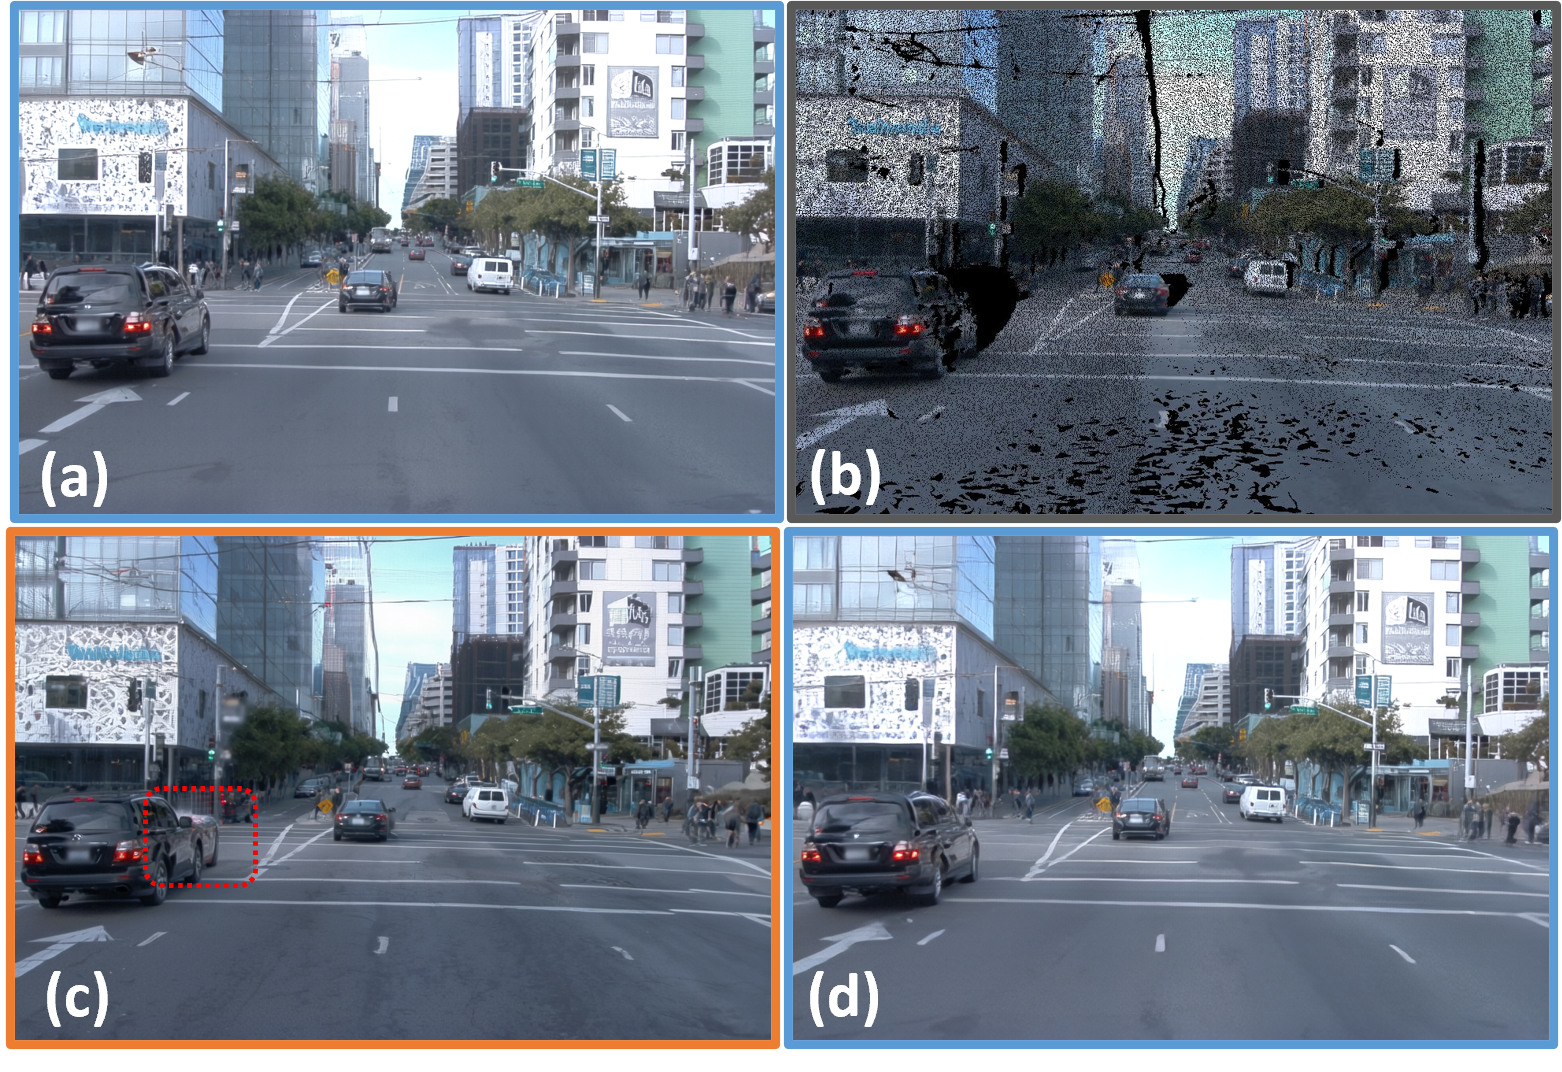
\includegraphics[width=\linewidth]{images/ablation_seg.png}
    \vspace{-0.25in}
    \caption{Ablation study on segment-wise video generation: (a) last frame of the previous segment; (b) first pseudo-novel view of the next segment; (c) view generated by the ablation model; (d) view generated by our default model. Compared to (c), (d) provides a much more coherent transition with (a).}
    \label{fig:Ablation_seg}
\end{figure}


% To assess the effect of segment-wise video generation in the coherent transitions between two segments, we train a variant where the first condition frame of each segment is also a simulated novel pseudo-view. This model generates all frames in a segment without reference to the last frame of the previous segment.
To assess the importance of segment-wise conditioning for coherent transitions between segments, we train a variant where the first conditioning frame of each segment is also a simulated pseudo-view rather than the last generated frame from the previous segment.
We test both models on two consecutive segments. Fig.~\ref{fig:Ablation_seg} shows: (a) the last frame of the previous segment, (b) the first novel pseudo-view of the next segment, (c) the view generated from (b) by the ablation model, and (d) the view generated from (b) by our default model. Our method yields smoother transitions and better visual consistency across segments, especially in regions with missing content, demonstrating the effectiveness of segment-wise anchoring.

\begin{table}[t]
  \centering
  \small
  \setlength{\tabcolsep}{6pt} % column separation for one-column width
  \begin{tabular}{lccc}
    \toprule
    Corruption & NTA-IoU $\uparrow$ & NTL-IoU $\uparrow$ & FID $\downarrow$ \\
    \midrule
    --                 & 0.558 & 56.83 & 49.77 \\
    $-20\%$ Gaussians  & 0.555 & 56.54 & 50.67 \\
    $-40\%$ Gaussians  & 0.542 & 56.02 & 51.75 \\
    $-80\%$ Gaussians  & 0.535 & 54.79 & 50.86 \\
    $\pm 0.1$ m noise  & 0.545 & 56.62 & 52.13 \\
    $\pm 0.2$ m noise  & 0.538 & 56.24 & 50.97 \\
    \bottomrule
  \end{tabular}
  \vspace{-0.1in}
  \caption{Performance under different corruptions. The first row is our default model without corruption}
  \label{tab:corruption_table}
  \vspace{-0.2in}
\end{table}

\paragraph{Robustness of Segment-wise Video Diffusion Model}
We evaluate the robustness of our Segment‑wise video diffusion model by corrupting the underlying 3D Gaussian representation to synthesize pseudo‑novel views with severe artifacts, and then requiring our video diffusion model to restore them. The corruption comprises two schemes: (i) randomly dropping a subset of Gaussian primitives and (ii) adding i.i.d. translation noise to each Gaussian’s x, y, and z coordinates. On the same test set as ~\cref{sec:comparison}, ~\Cref{tab:corruption_table} shows that removing up to 80\% of Gaussians or injecting uniformly sampled translation noise within ±0.2 m yields only marginal changes in final metrics.
% and Figure XXX illustrates that our video diffusion model corrects artifacts even when 80\% of Gaussians are dropped. 
These results demonstrate strong robustness, which we attribute to the model’s generalizability and the effectiveness of our pseudo‑view simulation pipeline. Please check the supplementary for additional visual results.





% This diffusion model is used to generate novel views of each segment separately. 

% We compare the results that generated 
% Figure[XXX] shows that  



% address the lack of depth information in regions not covered by LiDAR. To evaluate its effectiveness, we train models on the Waymo dataset with and without this supervision. As shown in ~\Cref{fig:Ablation_aligned}, the model trained without aligned depth supervision exhibits significant depth estimation errors, particularly in regions where LiDAR data is sparse or absent—such as the upper half of the scene or distant background areas. In contrast, the inclusion of aligned depth supervision substantially reduces these errors, demonstrating its effectiveness in improving geometry reconstruction in under-constrained regions.





% \vspace{-0.1in}
% \paragraph{Ablation Study on trajectory expansion mechanism}

% To analyze the impact of our progressive trajectory expansion strategy, we conduct an ablation study on a 2.5-meter leftward shift scenario. We evaluate the following configurations: (a) Direct shift of 2.5 meters in a single step. (b) Two-step shift, each of 1.25 meters.  (c) Three-step shift, each of approximately 0.83 meters. (d) Four-step shift, each of approximately 0.625 meters. As shown in the ~\Cref{fig:Ablation_Trajectory}, setting (d) produces the fewest visual artifacts and the most temporally consistent outputs. This validates the effectiveness of our progressive expansion strategy in maintaining visual fidelity during large trajectory shifts.